%%
%% This is file `example-1.tex',
%% generated with the docstrip utility.
%%
%% The original source files were:
%%
%% drexel-thesis.dtx  (with options: `example-part')
%% 
%% This is a generated file.
%% 
%% Copyright (C) 2010 W. Trevor King
%% 
%% This file may be distributed and/or modified under the conditions of
%% the LaTeX Project Public License, either version 1.3 of this license
%% or (at your option) any later version.  The latest version of this
%% license is in:
%% 
%%    http://www.latex-project.org/lppl.txt
%% 
%% and version 1.3 or later is part of all distributions of LaTeX version
%% 2003/06/01 or later.
%% 

\chapter{Quasi 2-D and 2.5-D Systems}

\section{Two-dimensional sheets of neurons}
Computational 2D systems: \citet{keane2015}\citet{Spreizer2019}

Bio 2D waves: \citet{huang2004}\citet{Townsend2018}

As we did with our quasi 1-D minicolumn, we first create a purely 2-D sheet of neurons with X=100, Y=100 and Z=1.
Model parameters are fixed at $\Sigma$.
We do not observe traveling waves or other spatiotemporal patterns in this system (Figure \ref{fig:Pure2DRasters_NoWaves}).
\begin{figure}[!htb]
 \caption{ Raster plots from our purely 2-D system do not show coherent spatiotemporal patterns.}
 \label{fig:Pure2DRasters_NoWaves}
 \centering
   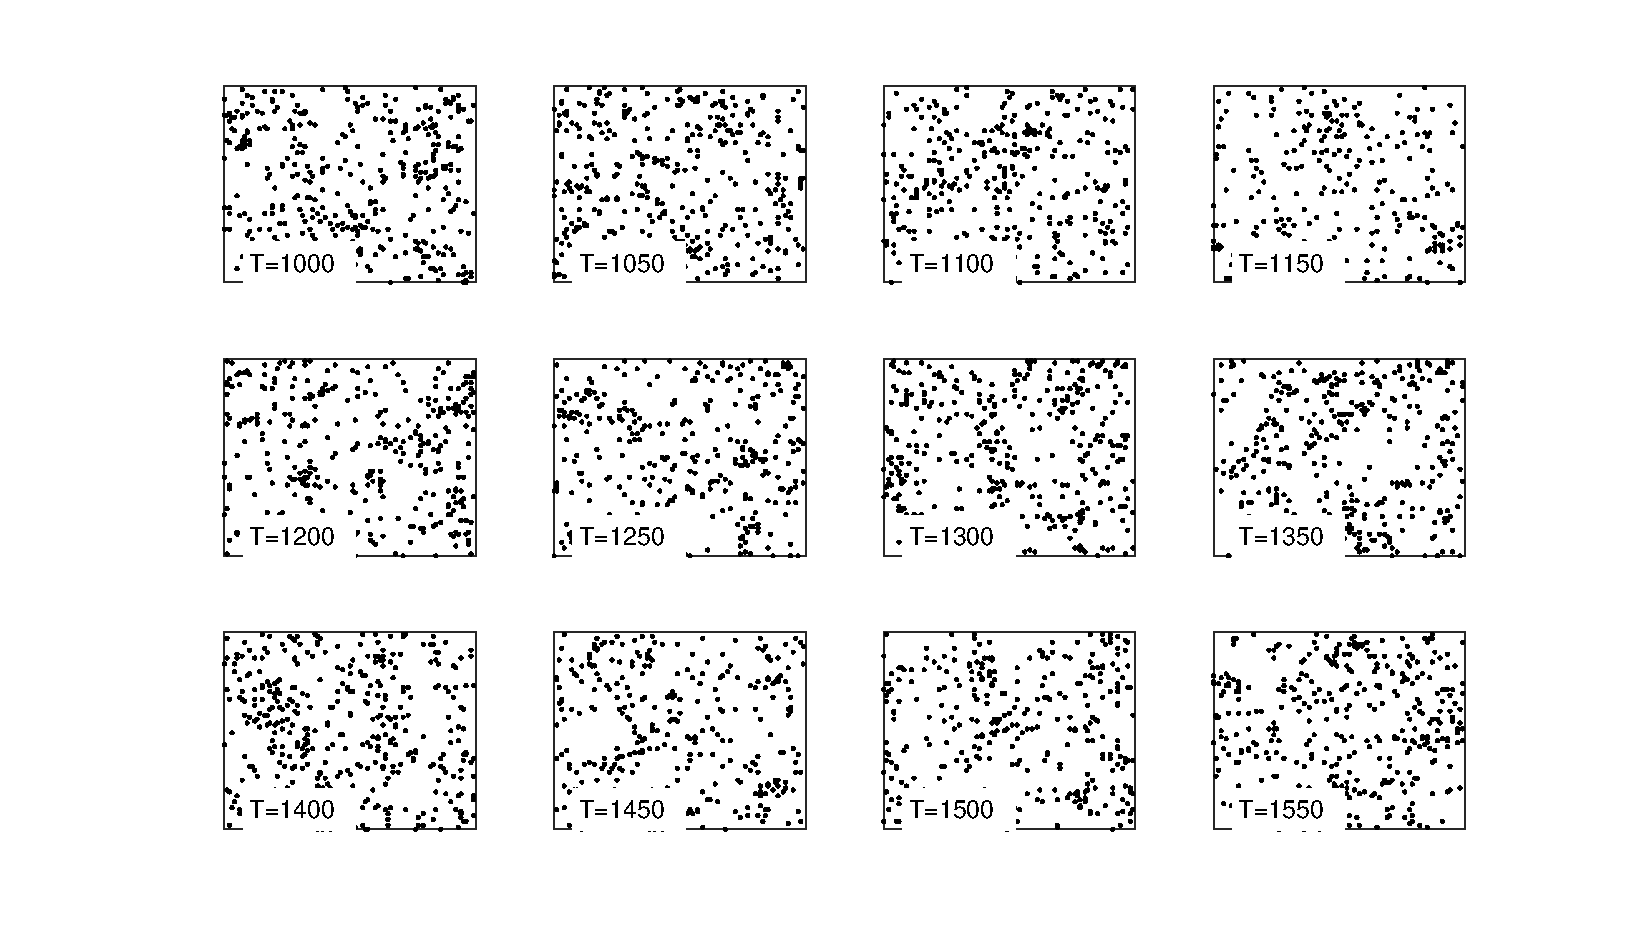
\includegraphics[width=\textwidth]{fig/2DWaveRasters_1LayerNoWaves}
\end{figure}

We then extend our system to a quasi 2-D sheet with X=100, Y=100 and Z=2.
We now observe traveling wave patterns in the system in Figure \ref{fig:2D_waves}.
These patterns emerge in spite of the high variability in the neuron types, neuron dynamics and connectivity present in our model.
\begin{figure}[!htb]
 \caption{ Raster plots from our quasi 2.5-D system with two layers show wave patterns that spread across the surface of the sheet.}
 \label{fig:2D_waves}
 \centering
   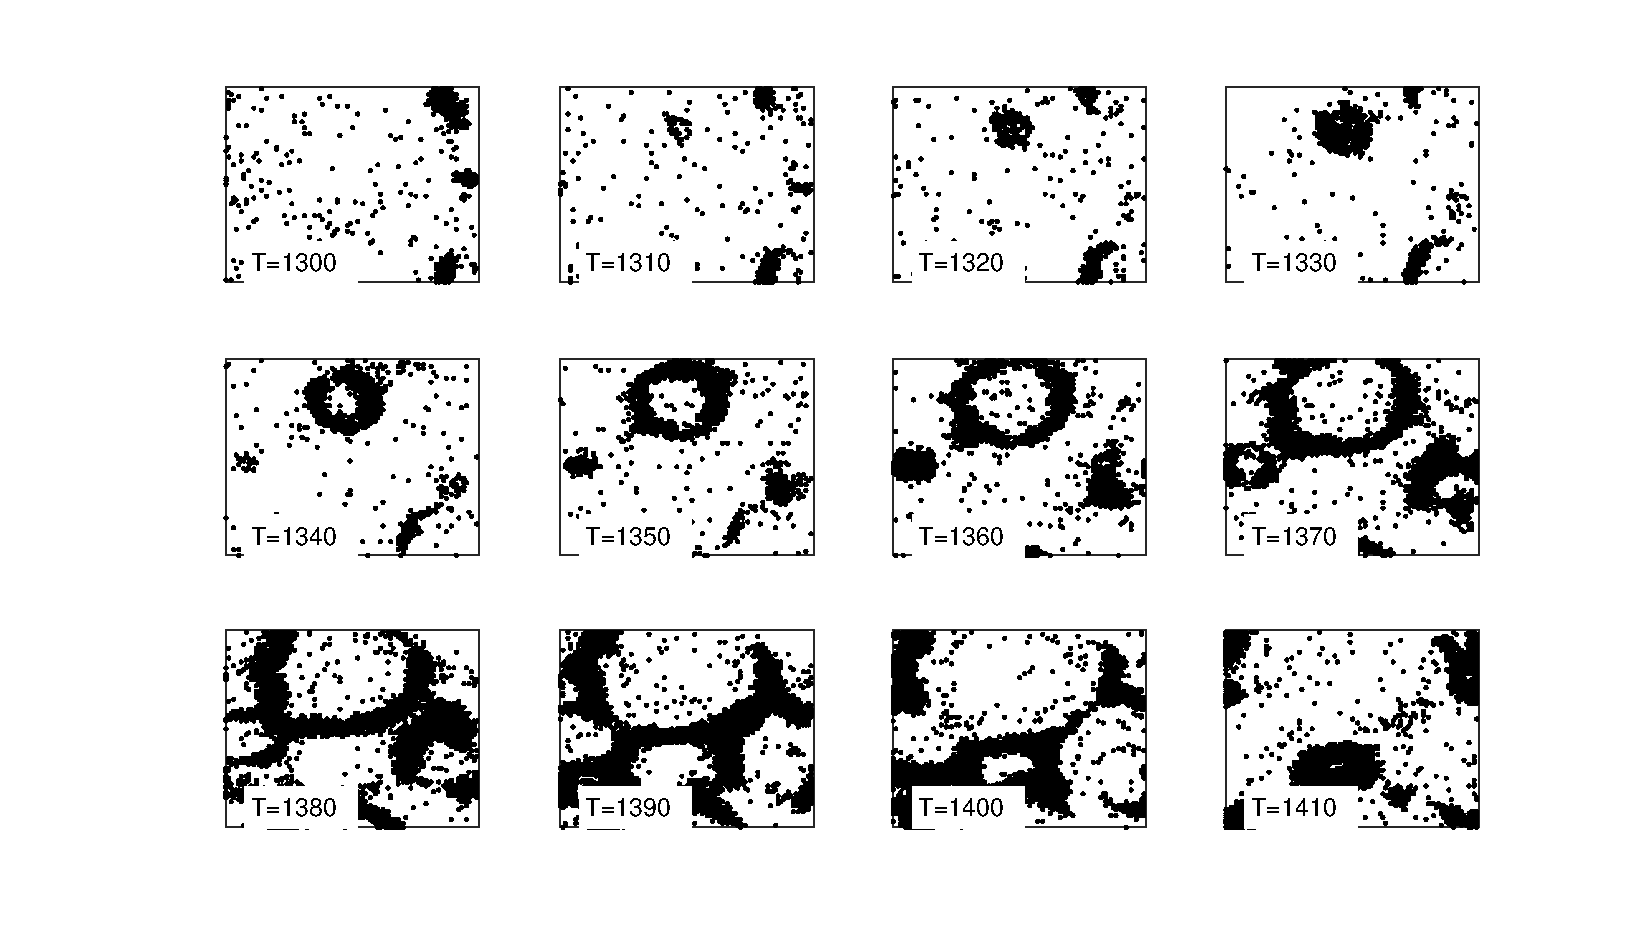
\includegraphics[width=\textwidth]{fig/2DWaveRasters}
\end{figure}

In some simulations we see the formation of large-scale plane waves across the entire system as seen by \citet{keane2015}.
In their work, plane waves were formed when excitation dominated their neuronal system.
The formation of these plane waves in our system does not seem deterministic, as a different random draw of the uniform background stimulus for the same neuronal system may not exhibit plane waves.
Nonetheless, these results show that plane waves can emerge as a stable pattern in systems of this type even when excitation does not dominate.
\begin{figure}[!htb]
 \caption{ Raster plots from our quasi 2.5-D system showing large-scale plane waves moving from top to bottom.}
 \label{fig:2D_plane_wave}
 \centering
   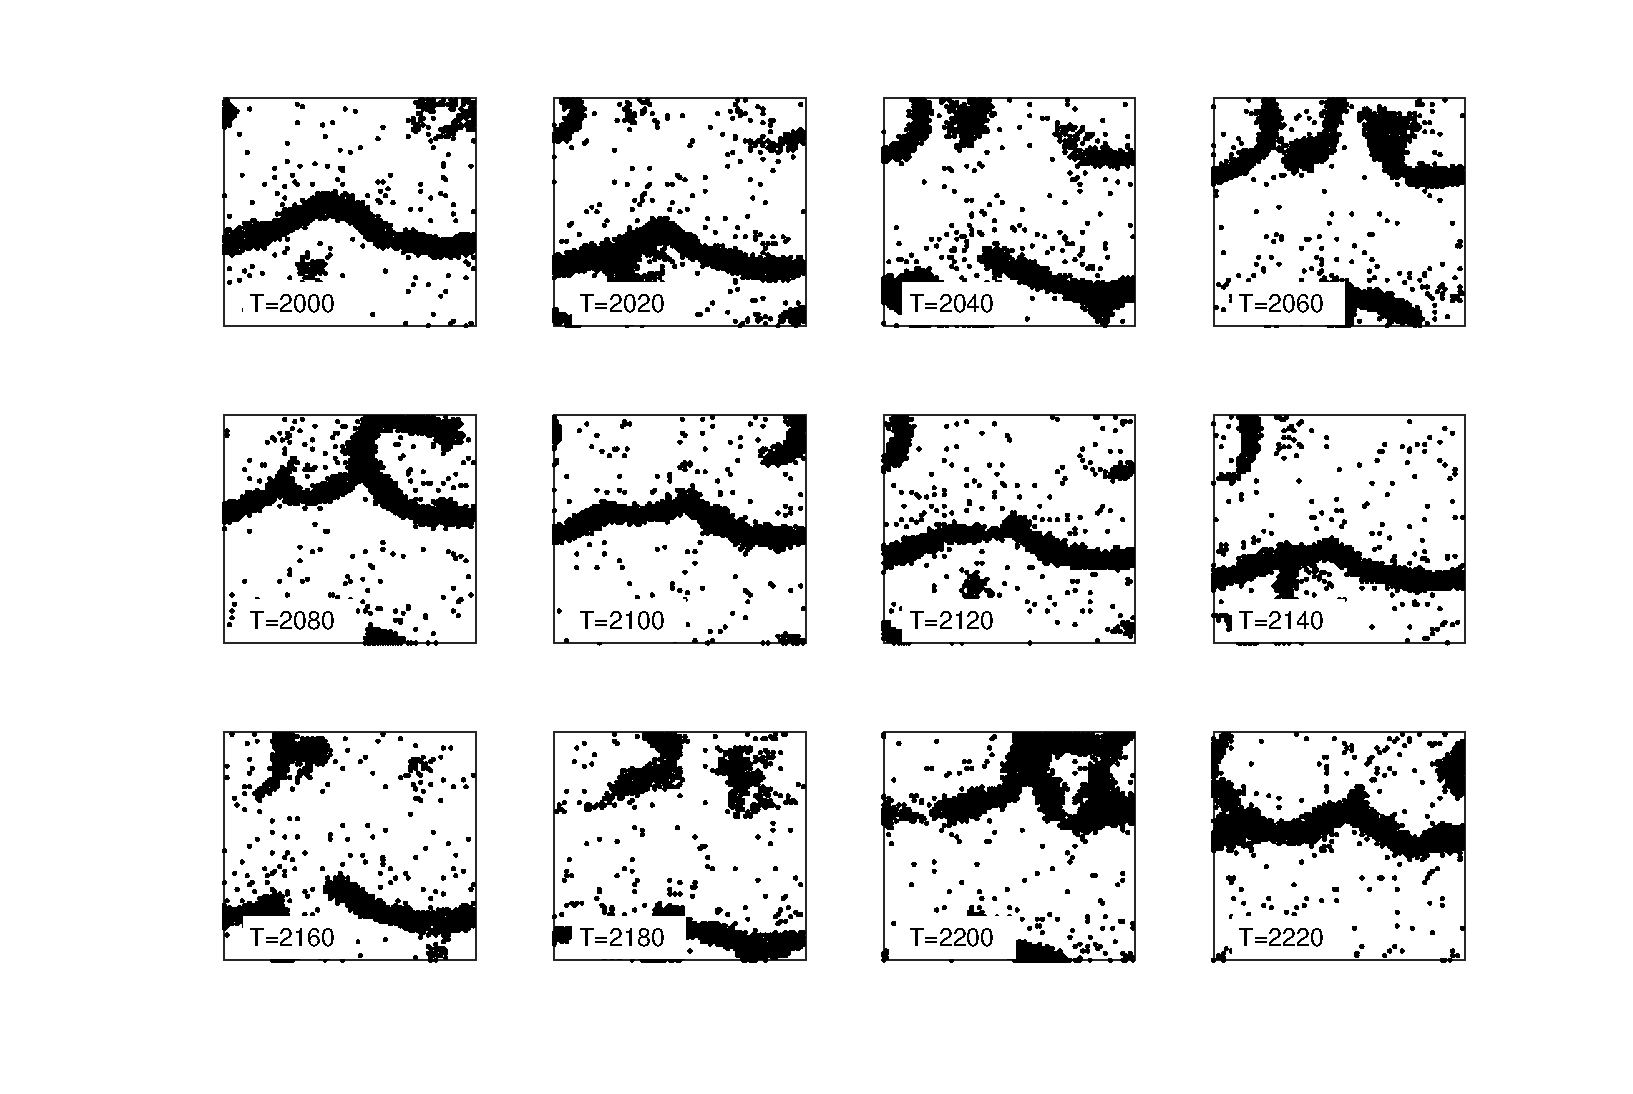
\includegraphics[width=\textwidth]{fig/2DWaveRasters_PlaneWave}
\end{figure}

\FloatBarrier

In \citet{keane2015} traveling waves in 2-D sheets were proposed to explain simultaneous spike timing irregularity with fluctuations in the average firing rate of the ensemble. 
Despite the complex spatiotemporal patterns the overall mean voltage shows a small, steady oscillation.
\begin{figure}[!htb]
 \caption{ After initial fluctuations settle out, the system mean voltage settles into small oscillations.}
 \label{fig:2D_mean_voltage}
 \centering
   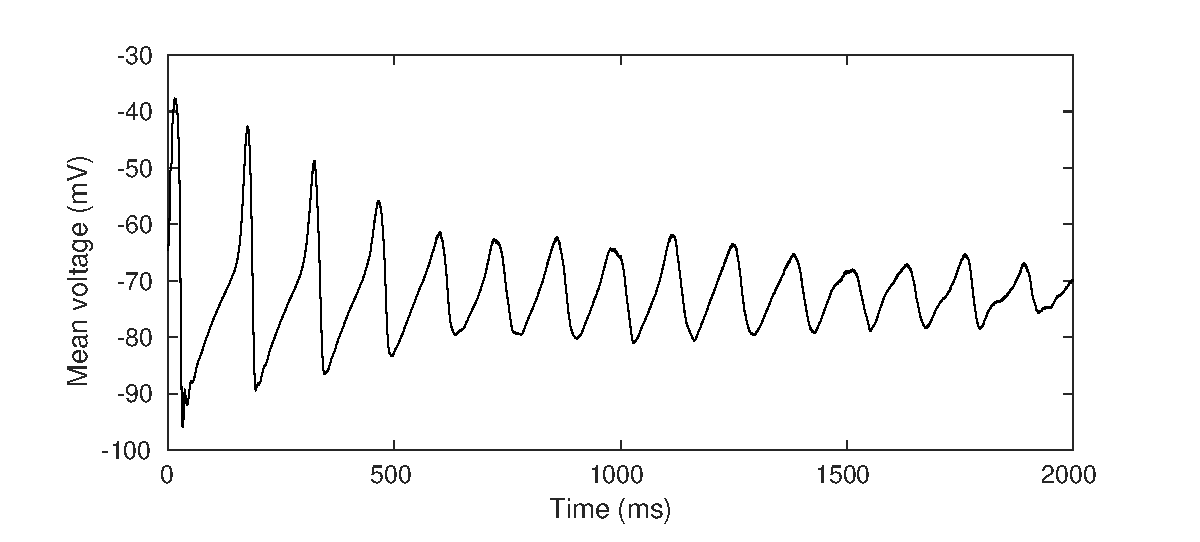
\includegraphics[width=\textwidth]{fig/MeanVoltage_PBC}
\end{figure}


\FloatBarrier
\section{Ensembles of minicolumns}
In section 3.2 we showed that as SCE grow in the X or Y dimension the wave speed increases due to the increased connectivity, but when the average number of connections per neuron were held constant the wave speed was constant.
We further examine these thicker, but still quasi one-dimensional SCE by examining the firing activity of purely one-dimensional sub-columns within the larger SCE (with topology 2x2x100 extracted from the central core of the thicker SCE, away from the surfaces, except of course for the 2x2 and 3x3 SCEs).
With the average number of connections held constant, the sub-columns within the larger SCE show similar firing fraction with $K$ regardless of the overall topology (Figure \ref{fig:LargeSCESubcolumns}).
We remark that as the X and Y extents increase, the behavior seems to change from traveling waves to more synchronized firing activity.
This behavior as a function of width suggests that the system dynamics transition from supporting traveling waves to a system that exhibits global synchrony.
\begin{figure}[!htb]
 \caption{ Spike raster plots for complete SCE (A) and one-dimensional sub-columns (B) for different topologies show similar firing patterns in the sub-columns regardless  of topology. 
           The wave firing fraction (C) measured within the sub-columns show the same dependence on $K$ regardless of the topology.}
   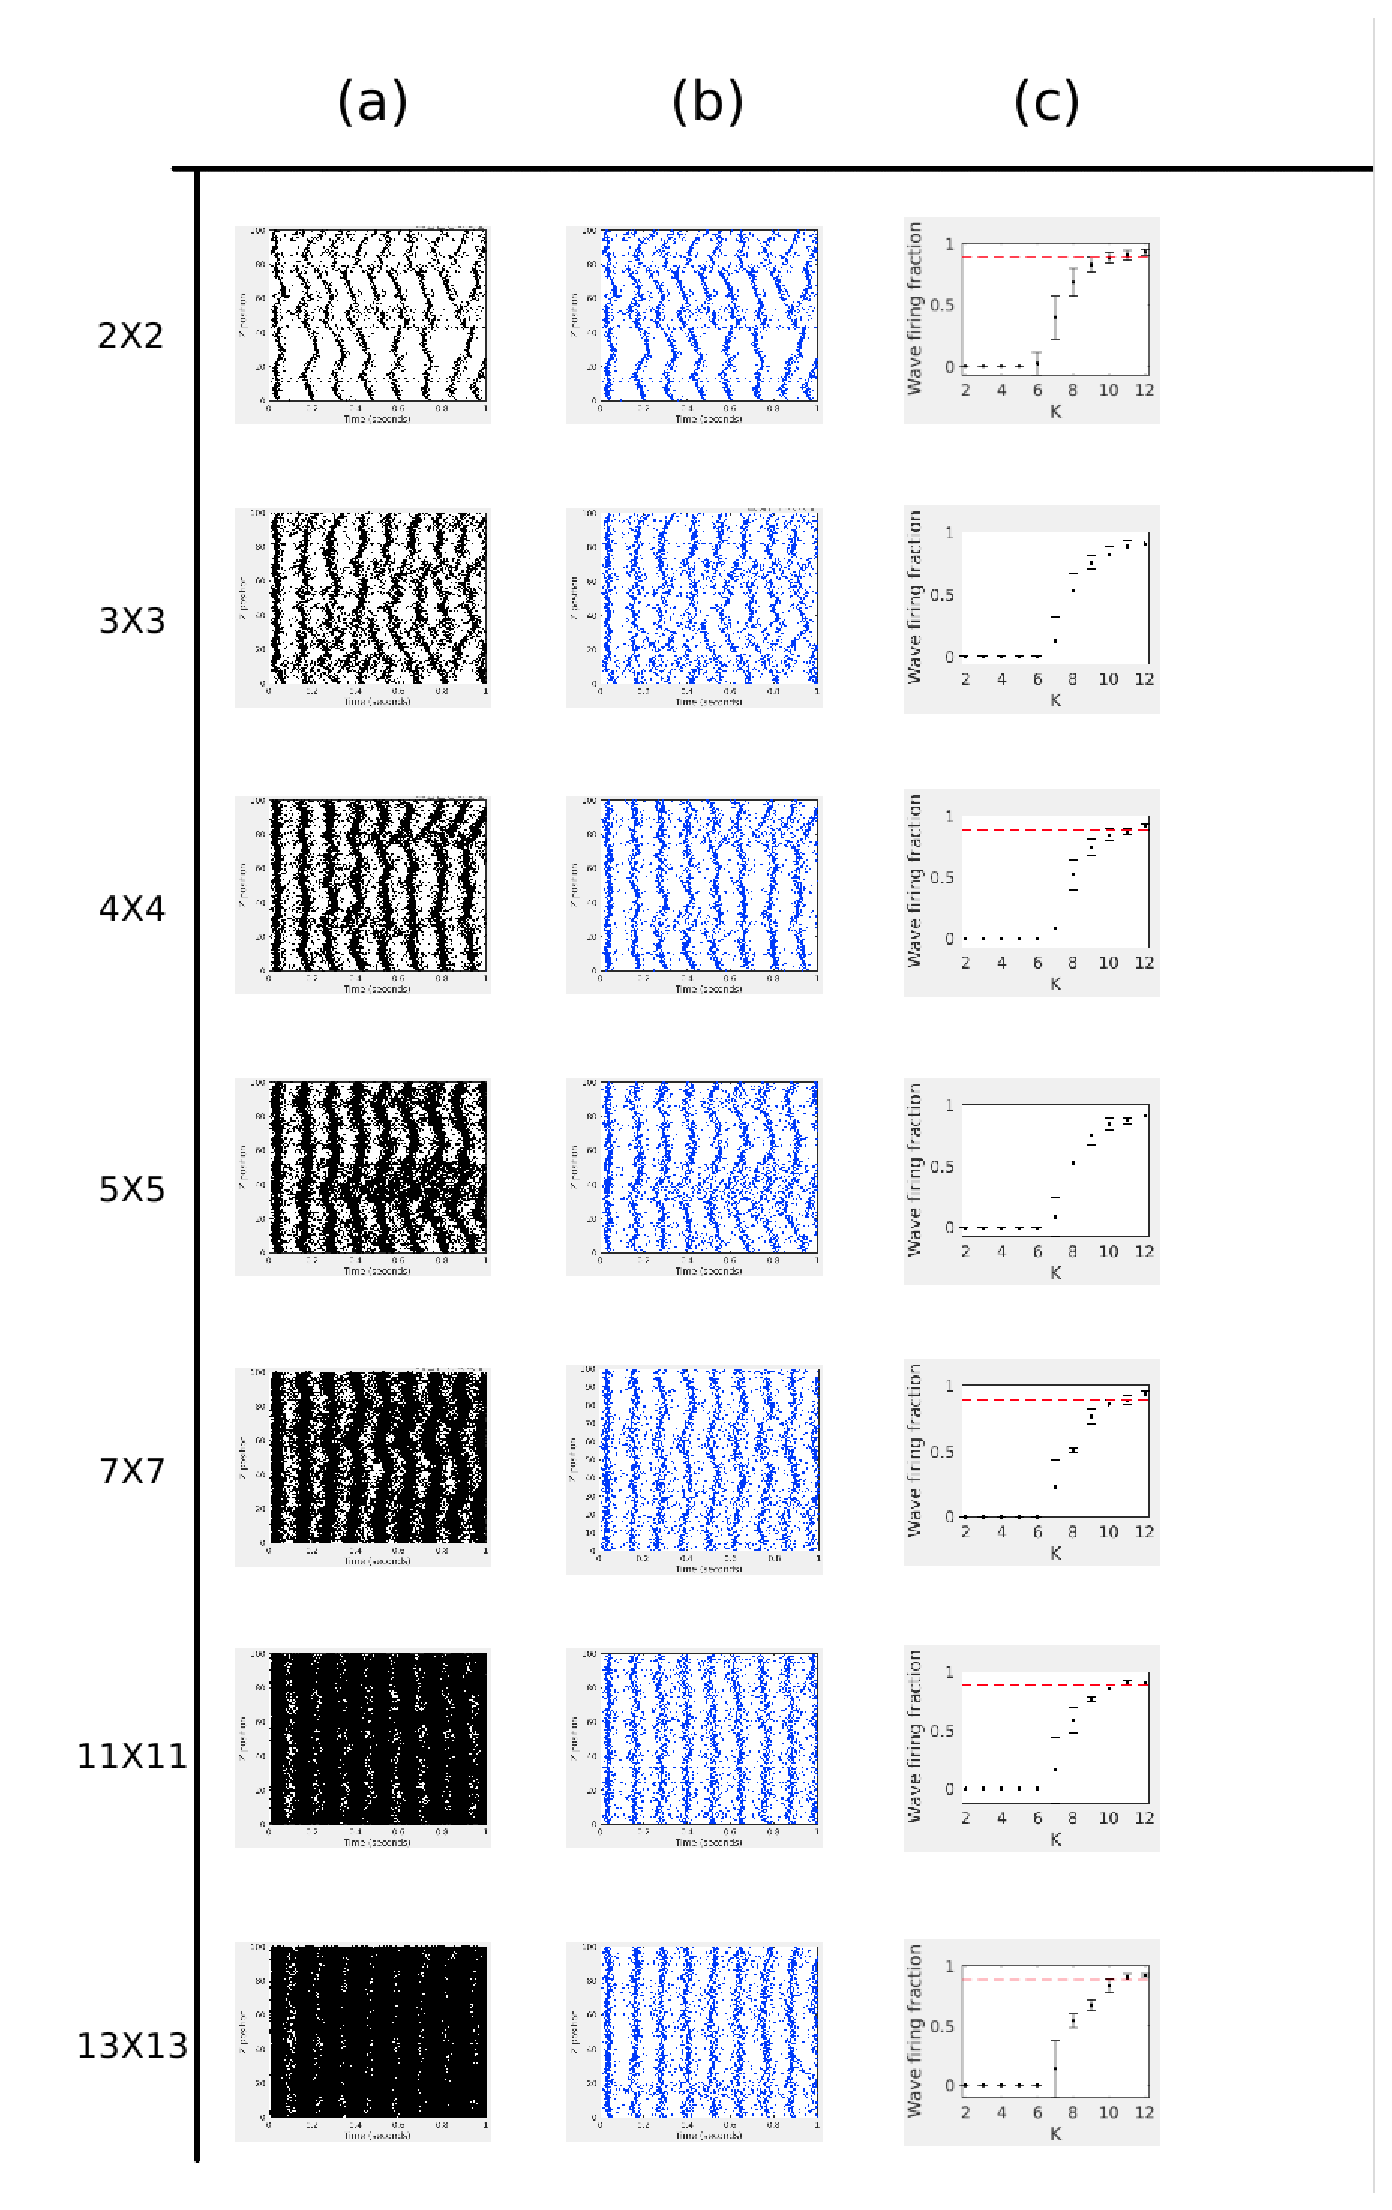
\includegraphics[width=0.75\textwidth]{fig/WaveFractionVsThick}
   \label{fig:LargeSCESubcolumns}
\end{figure}
\FloatBarrier



\FloatBarrier


\endinput
%%
%% End of file `example-1.tex'.
